\chapter{Project 4: blinking LED with memory access}
So far, the PL and PS parts of the SoM have been exploited separately, without actually interconnecting them so as to control or to communicate with the programmable logic through the system processor. Within this project, more focused is given into the development of design that allows to read a specific memory address in order to communicate with the system processor. To do so, a specific component has been used, which allocate a defined memory address to which R/W operations can be performed.


\section{Vivado project}
Figure \ref{fig:prj4_1} shows the design block scheme of the project. The system processor was set either by applying the procedure linked in the previous chapter or by starting from the fan design example.
\begin{figure}[ht]
	\centering
	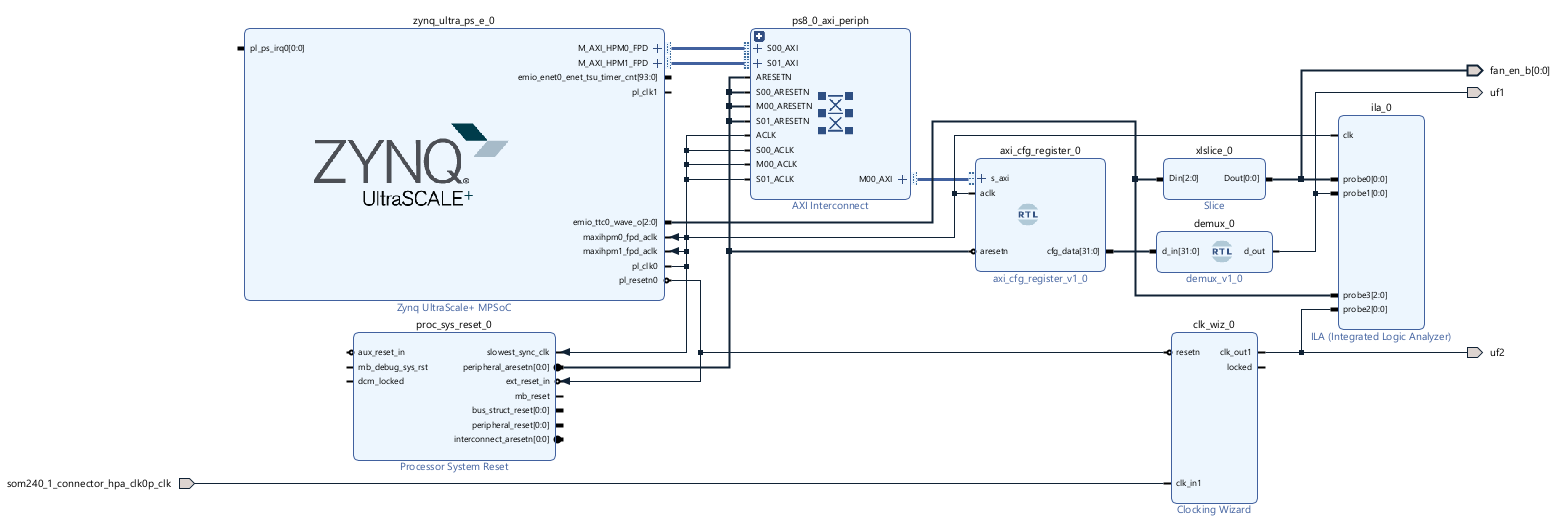
\includegraphics[width=\textwidth]{images/prj4_1}
	\caption{Block Design Layout.}
	\label{fig:prj4_1}
\end{figure} 
From the \textbf{Address Editor} window, the memory space reserved for this application was set to be 128bit (there is no need for higher space, since only a bit is needed to be read and written) and the memory address to $0xB0000000$. 
\begin{figure}[ht]
	\centering
	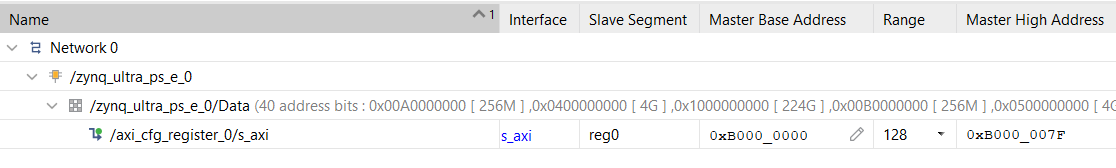
\includegraphics[width=\textwidth]{images/prj4_2}
	\caption{Address editor.}
	\label{fig:prj4_2}
\end{figure}
The component used to perform R/W operations is named \textit{axi\_cfg\_register}. As always, after having generated the bitstream, it is needed to export the hardware including the bitstream with it. Also the creation of the Petalinux project is not different from the previous. What changes is the procedure after the boot of the board.



\section{Code implementation}
After having successfully created and built the project, to perform R/W operations on the memory allocated by the cfg\_register, there is the necessity to define a) the driver and b) the program with which the operations are performed.

\subsection{Driver}
The generation of the driver is beyond the scope of this guide. It is assumed that the corresponding .c and .h files are already available. In this discussion it is explained how to create a driver needed to blink the led, but the same procedure can be applied to a wide variety of applications. Now, assuming the .c and .h files are respectively named 
\begin{verbatim}
	driver_name.c
	driver_name.h
\end{verbatim}
then, the creation of the driver modules is performed with the command
\begin{verbatim}
	petalinux-create -t modules --name driver_name --enable
\end{verbatim}
after which 
\begin{verbatim}
	petalinux-build -c driver_name
\end{verbatim}
will build the module. Now, the aforementioned files .c and .h are to be copied into the \textit{project-spec/meta-user/recipes-modules/driver\_name/files/} path. Finally, to build the module
\begin{verbatim}
	petalinux-build -c driver_name
\end{verbatim}
\subsection{C program}

\section{Board booting}

\section{J-TAG debugging}

